\newpage
\section{Teknisk verkemåte}
\thispagestyle{fancy}
Sande reinseanlegg er konstruert og basert på \gls{SBR}-teknologi.

\gls{SBR} står for ``Sequence \Gls{Batch} Reactor'', på norsk ``sekvensiell \gls{Batch}reaktor''.\newline
\gls{SBR} er en reinsemetode der alle prosessar føregår i same reaktortank. 
Reaktor nyttar biologisk reinsing, ved hjelp av aktivert slam som inneheld mikroorganismar, for å koagulere 
og å fjerne løyste og ikkje sedimenterbare partiklar, samt stabilisere organisk materiale. 
Avlaupsvatn tilførast reaktor i ``\gls{Batch}er'' for å bli behandla. 
Kvar avlaups-\gls{Batch} går gjennom ein reaktorsyklus som består av følgjande fem delsekvensar \citep{Statsforvalter}.
\newline

\begin{figure}[htbp]
    \centering
    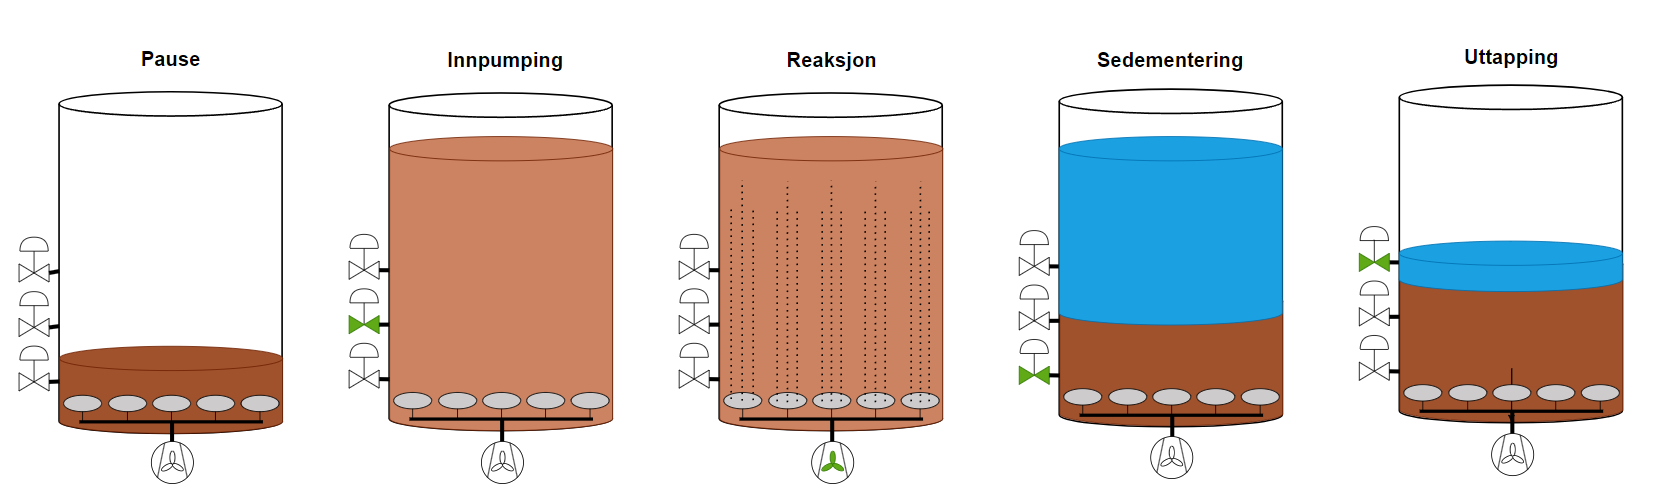
\includegraphics[width=1\textwidth]{Figurar/SBR-V2.png}
    \caption{\gls{SBR}-prosessen}\label{fig:SBR-Prosessen}
\end{figure}


\begin{enumerate}
    \item \textbf{\makebox[3cm][l]{Pause}:} Reaktor er klar og ventar.
    \item \textbf{\makebox[3cm][l]{Innpumping}:} Reaktor mottar avlaupsvatn, normalt frå ein utjamningstank.
    \item \textbf{\makebox[3cm][l]{Reaksjon}:} Reaktor luftast periodisk for å tilføre oksygen til mikroorganismane.
    \item \textbf{\makebox[3cm][l]{Sedimentering}:} Reaktor sedimenterer ved hjelp av gravitasjon. Overskuddslam fjernast.
    \item \textbf{\makebox[3cm][l]{Uttapping}:} Reaktor drenerar reinsa vatn mot resipient.
\end{enumerate}

Meir detaljert informasjon om \gls{SBR} og anleggets teknologiske prinsipp er tilgjengeleg, via vedlegg, i anleggets nye
funksjonsbeskrivelse. (Vedlegg A)

